Large language model (LLM) agents are increasingly utilized in financial analysis to answer questions in regulatory filings~\citep{islam2023financebench,chen2021finqa,reddy2024docfinqa}, carry out multi-step research and retrieval over corporate disclosures~\citep{bigeard2025financeagent,choi2025finagentbench,krumdick2024bizbench,xie2024finben}. The agent reads a user's question, searches through relevant filings and returns the answer for downstream actions. 

However, financial questions are often deceptively under-specified. Financial terminology is highly specific, and a natural language question may map to several defensible readings for different numbers, e.g. in the question \emph{``What was Meta Platforms' operating income?''} (Figure~\ref{fig:teaser}), an agent must decide whether the user means the consolidated GAAP figure (\$46.75B for FY2023) or the Family of Apps segment (\$62.87B), both being programmatically verifiable against SEC facts. A capable agent should recognize the ambiguity and follow up with the user instead of directly committing into a plausible but unintended reading. 

Existing financial benchmarks cannot measure this as they grade only the final answer by assuming the question is disambiguated~\citep{islam2023financebench,chen2021finqa,reddy2024docfinqa,krumdick2024bizbench,xie2024finben}. Without grounding check, they cannot distinguish whether the agent actually resolves the ambiguity or guesses the common reading. We call such blind spot \emph{single-gold illusion} (Table~\ref{tab:comparison}), which is currently underexplored in the financial domain relative to general ambiguous QA literature~\citep{min2020ambigqa,li2025condambigqa,kuhn2022clam}. We study financial ambiguity over three research questions: \begin{itemize}[leftmargin=*, topsep=3pt, itemsep=1pt, parsep=0pt]
    \item \textbf{RQ1}: Do frontier models recognize financial report ambiguity? 
    \item \textbf{RQ2}: What financial ambiguity leads to most failures?
    \item \textbf{RQ3}: Can we incorporate interventions at inference time to improve resolution?
\end{itemize}

\begin{figure*}[t]
\centering
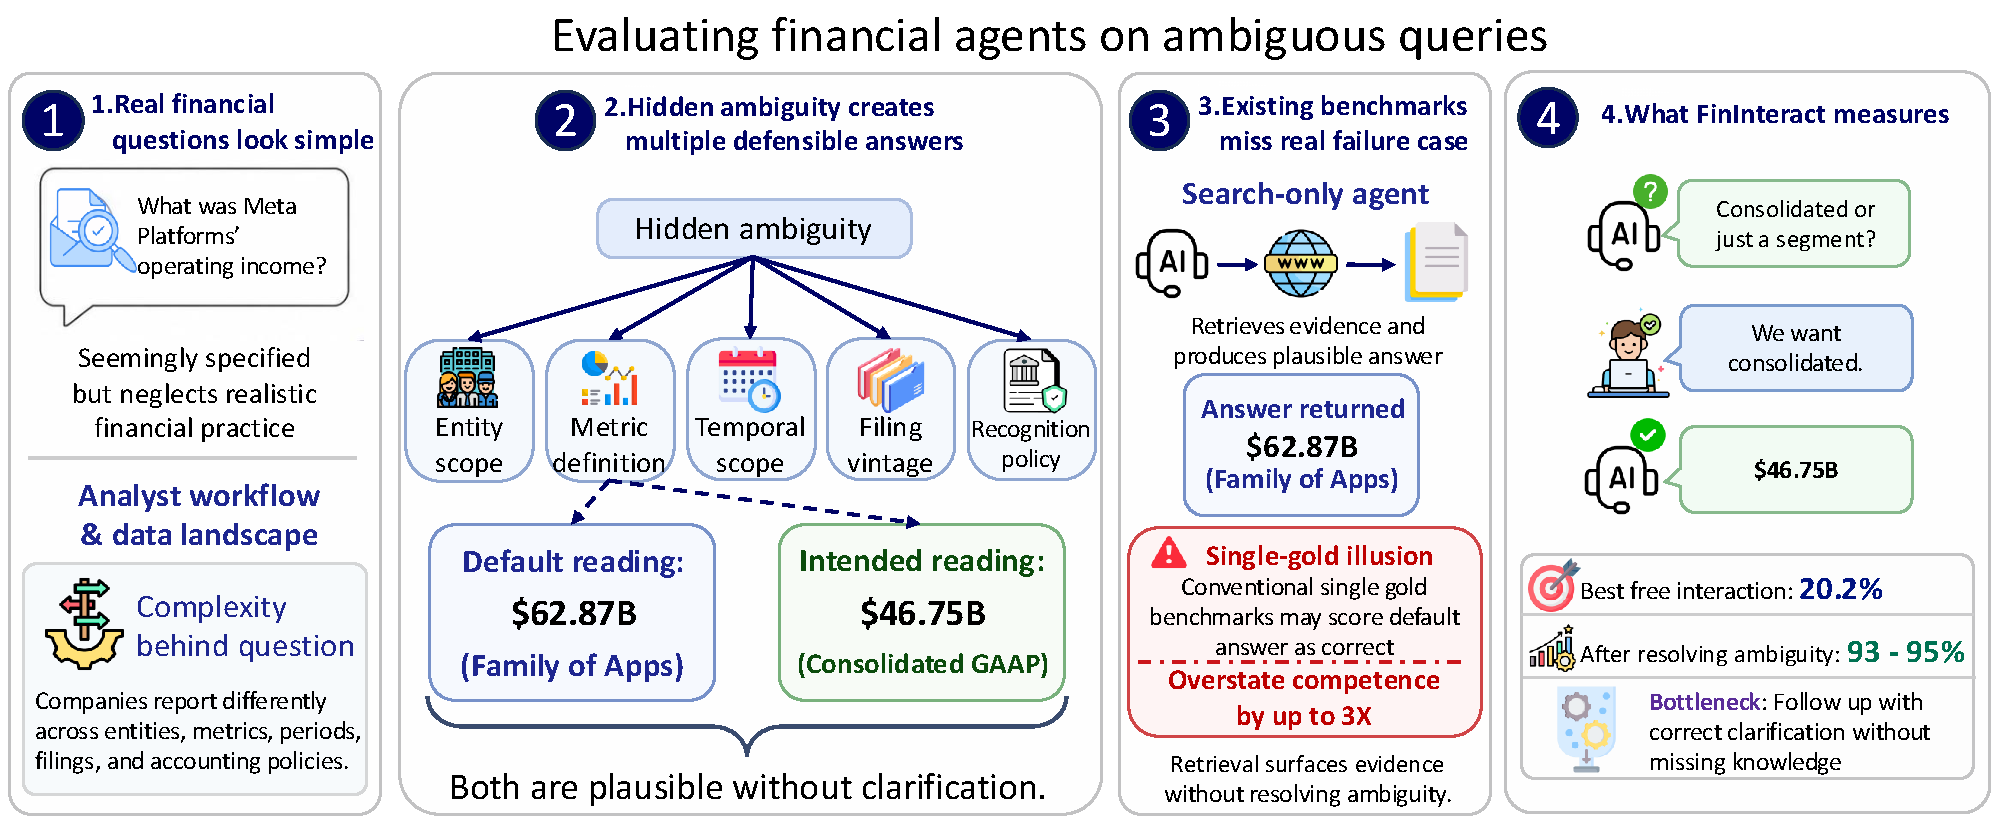
\includegraphics[width=\textwidth]{motivation_plot.pdf}
\caption{\textbf{Evaluating financial agents on ambiguous queries.}
\textbf{(1)}~A real analyst query (``What was Meta Platforms' operating income?'') looks
fully specified, but neglects that companies report differently across entities, metrics,
periods, filings, and accounting policies. \textbf{(2)}~The query hides ambiguity along five
categories (entity scope, metric definition, temporal scope, filing vintage, recognition policy),
here yielding two defensible answers, a default reading of \$62.87B (Family of Apps segment)
and the intended \$46.75B (consolidated GAAP), both plausible without clarification.
\textbf{(3)}~A search-only agent retrieves evidence and returns the plausible default, which
a conventional single-gold benchmark scores as correct, the \emph{single-gold illusion} that
overstates competence by up to $3\times$. \textbf{(4)}~\fininteract instead measures whether
an agent resolves the ambiguity by asking: for the GPT-5 agent shown, free-interaction
accuracy is $20.2\%$ while accuracy once the ambiguity is resolved is $93$--$95\%$, so the
bottleneck is issuing the right clarification without missing knowledge.}
\label{fig:teaser}
\end{figure*}

\begin{table}[h]
\centering
\caption{Running example: a \fininteract instance.
The paired default and intended readings are shown; $H_0{=}\log_2 3{\approx}1.58$ reflects
three plausible entity scopes for this question (consolidated total and two reportable
segments). Without the disambiguating context $C$, a model's default interpretation
leads to the wrong answer.}
\label{tab:example}
\small
\resizebox{0.9\columnwidth}{!}{%
\begin{tabular}{p{1.8cm}p{5.7cm}}
\toprule
Field & Value \\
\midrule
$Q$ &
  What was Meta Platforms' operating income? \\
$C$ &
  Total company (consolidated) results under U.S.\ GAAP for the year
  ended December 31, 2023. \\
$A$ (intended) &
  \$46.75B \emph{[consolidated GAAP]} \\
$A_d$ (default) &
  \$62.87B \emph{[Family of Apps segment]} \\
\midrule
Ambiguity category & Entity scope \\
$H_0$ & 1.58 bits \\
\midrule
Intended span &
  ``Income from operations for 2023 was \$46.75 billion\ldots'' \\
Default span &
  ``Family of Apps\ldots Income from operations \$62,871\ldots'' \\
\bottomrule
\end{tabular}}
\end{table}

Answering these questions requires three design properties. First,
the benchmark must draw representative ambiguity from real filings. Second, it must expose fine-grained dimensions of ambiguity through paired default and intended readings. Third, benchmark construction should have low cost and is safe from potential leakage to keep answer out of disambiguating context, with verifiable ground truth validated by domain experts. (Sec. \ref{sec:task}).

We release \fininteract, a bilingual benchmark in English and Chinese containing 173 instances, classified into five financial ambiguity categories. Each question $Q$ is paired with a \emph{default} interpretation recording a possible non-expert assumption and an \emph{intended} interpretation fixed by the disambiguating context. By grading the same model outputs against the default and intended interpretations, we effectively expose this single-gold illusion. \fininteract includes skill metric to localize which clarification ability the model lacks, and evaluates the agents under a ReAct protocol where the user simulator answers only from the disambiguating context (Figure~\ref{fig:framework}) to measure the agent's quality of clarify-then-integrate action. 

Our evaluation answers the research questions in turn. First, while frontier models detect ambiguity, they rarely resolve it effectively, as they ask the correct clarification question but still \textbf{failing to convert into the correct answer at the end} (Sec. \ref{sec:skills}). Second, \textbf{policy-related ambiguities} are the least resolved, as none of the proprietary models would initiate clarifications when facing this sparse category. Third, \textbf{inference intervention facilitates ambiguity resolution}, increasing accuracy from about 44\% to above 90\%, suggesting that this benchmark is not only diagnostic but also actionable. (Appendix~\ref{app:findings}). This paper makes three contributions \begin{enumerate}[leftmargin=*,itemsep=1pt]
  \item \textbf{Problem definition.} We formalize ambiguity in financial questions with five categories grounded in standard accounting and disclosure practice (Sec. \ref{sec:task}).
  \item \textbf{Benchmark.} We introduce \fininteract, a bilingual financial ambiguity dataset containing 173 instances, each paired with a default and an intended interpretation verified by domain experts. (Sec. \ref{sec:methodology}).
  \item \textbf{Empirical findings.} Our evaluation shows that existing models commonly fail to return correct final answer even when they have correctly clarified the intention, which can be improved via intervention at inference time. (Sec. \ref{sec:exp}).
\end{enumerate}
